\documentclass[a4paper ]{article}
\usepackage{graphicx}
\usepackage[letterpaper, landscape, margin=2in]{geometry}
\geometry{
	paper=a4paper, % Change to letterpaper for US letter
	inner=0.5cm, % Inner margin
	outer=0.5cm, % Outer margin
	bindingoffset=0.01cm, % Binding offset
	top=0.5cm, % Top margin
	bottom=0.5cm, % Bottom margin
	%showframe, % Uncomment to show how the type block is set on the page
}
\usepackage[utf8]{inputenc}
%\usepackage{natbib}

\begin{document}
- - -

\vspace{50mm}
\begin{center}
{\Huge \textsc{\textbf{Modelos Theta:}}}\\
{\Huge \textsc{\textbf{Comparando las Thetas de Hits y FA por clase}}}\\
\vspace{20mm}
\end{center}

\begin{center}
\textit{\huge Estudios en Detección de Señales - Tesis de Licenciatura}\\
\bigskip
\end{center}

\begin{center}
\textit{\huge Adriana F. Chávez De la Peña}\\
\end{center}

\begin{center}
\vfill
\textit{\huge adrifelcha@gmail.com}\\
\end{center}

\newpage



---
\begin{center}
{\LARGE \textbf{EXPERIMENTO 1} }\\
{\small \textsc{(Figura de Ebbinghaus vs Círculo))}}\\
\end{center}
\begin{figure}[h]
\centering
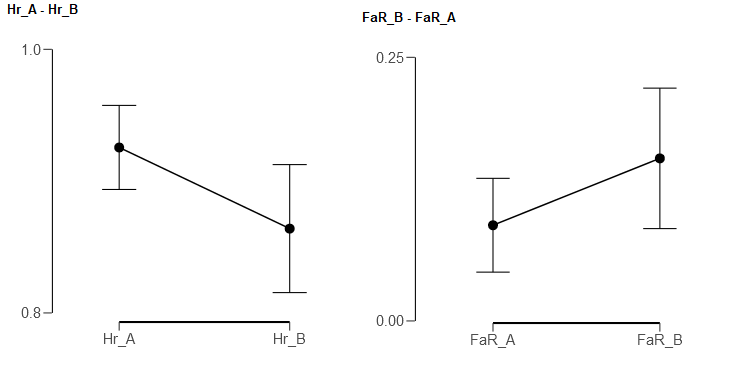
\includegraphics[width=.8\textwidth]{Figures/JASP_Ex1_Dispersion_HyFA}
\end{figure}
\clearpage


---
\begin{figure}[h]
\centering
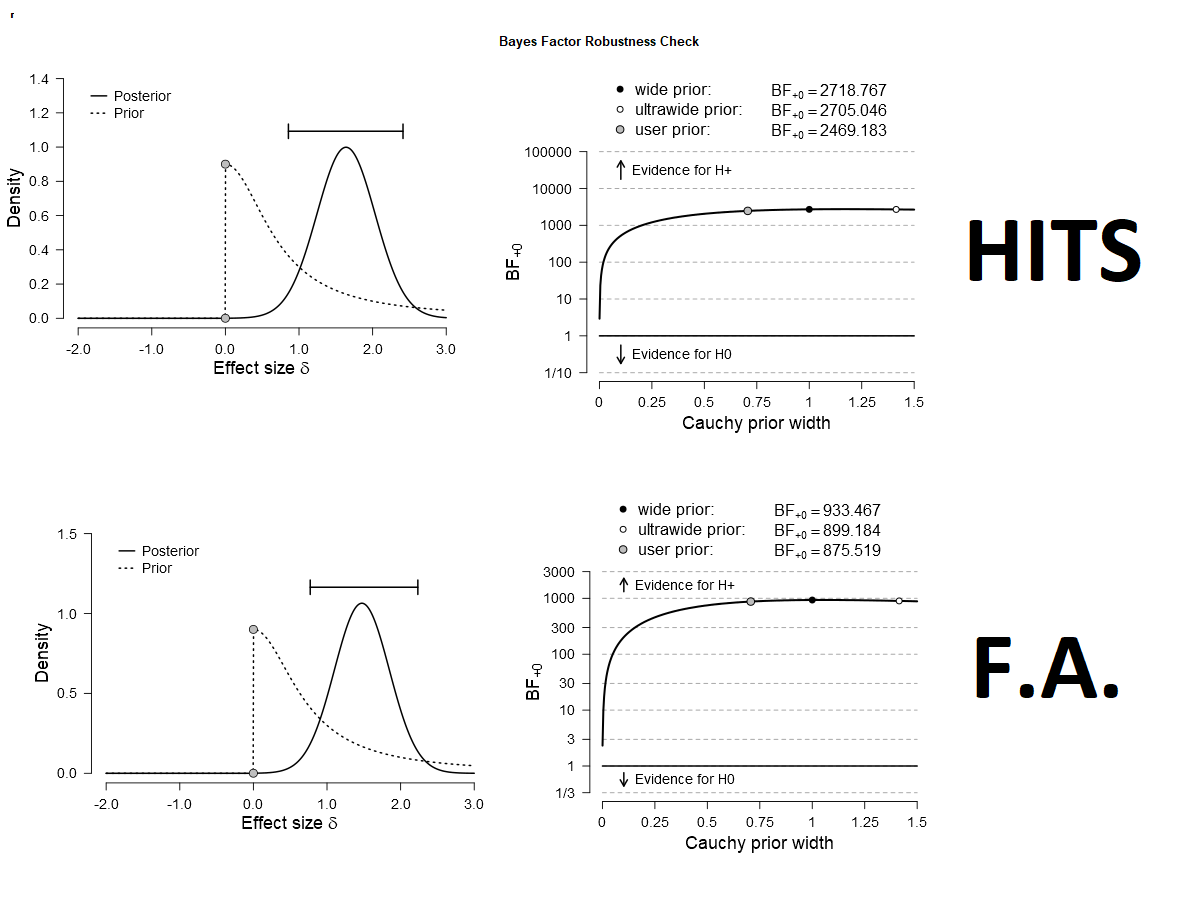
\includegraphics[width=.75\textwidth]{Figures/JASP_Ex1_tTest_HyFA}
\end{figure}
\clearpage


---
\begin{center}
{\LARGE \textbf{Modelo gráfico 1:} }\\
{\small \textsc{(El parámetro Tau estima la diferencia entre las ThetaH y Theta FA))}}\\
\smallskip
\end{center}

\begin{figure}[h]
\centering
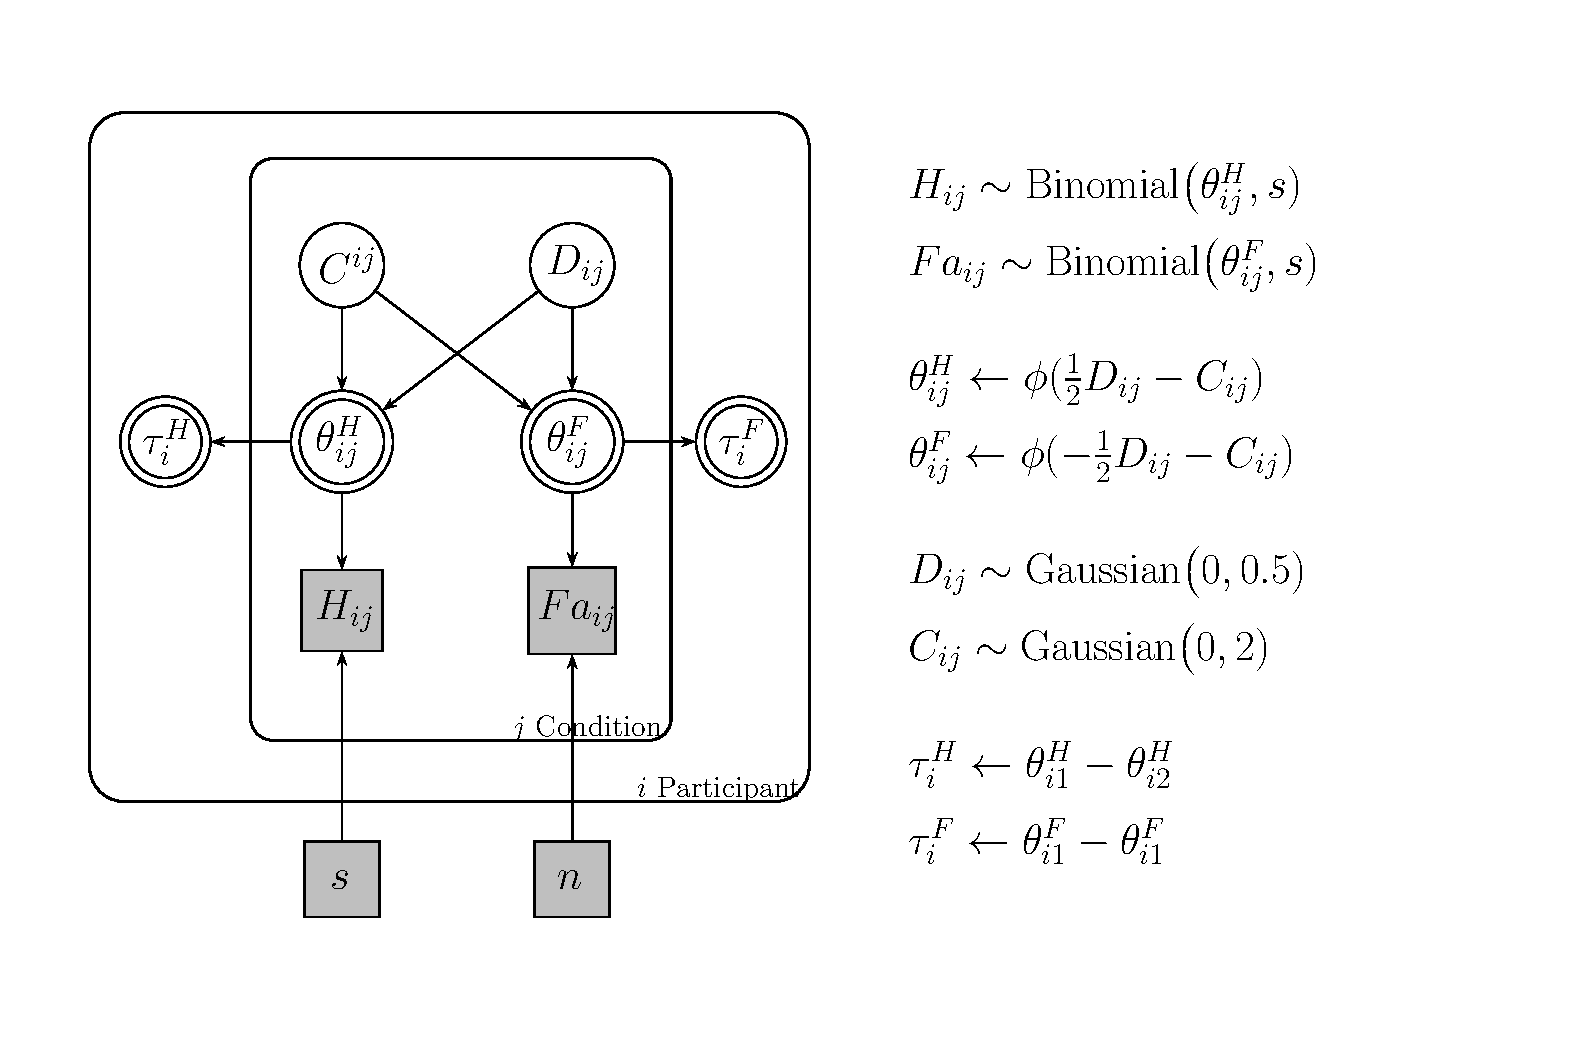
\includegraphics[width=.8\textwidth]{Figures/Theta_Tau}
\end{figure}
\clearpage


---
\begin{figure}[h]
\centering
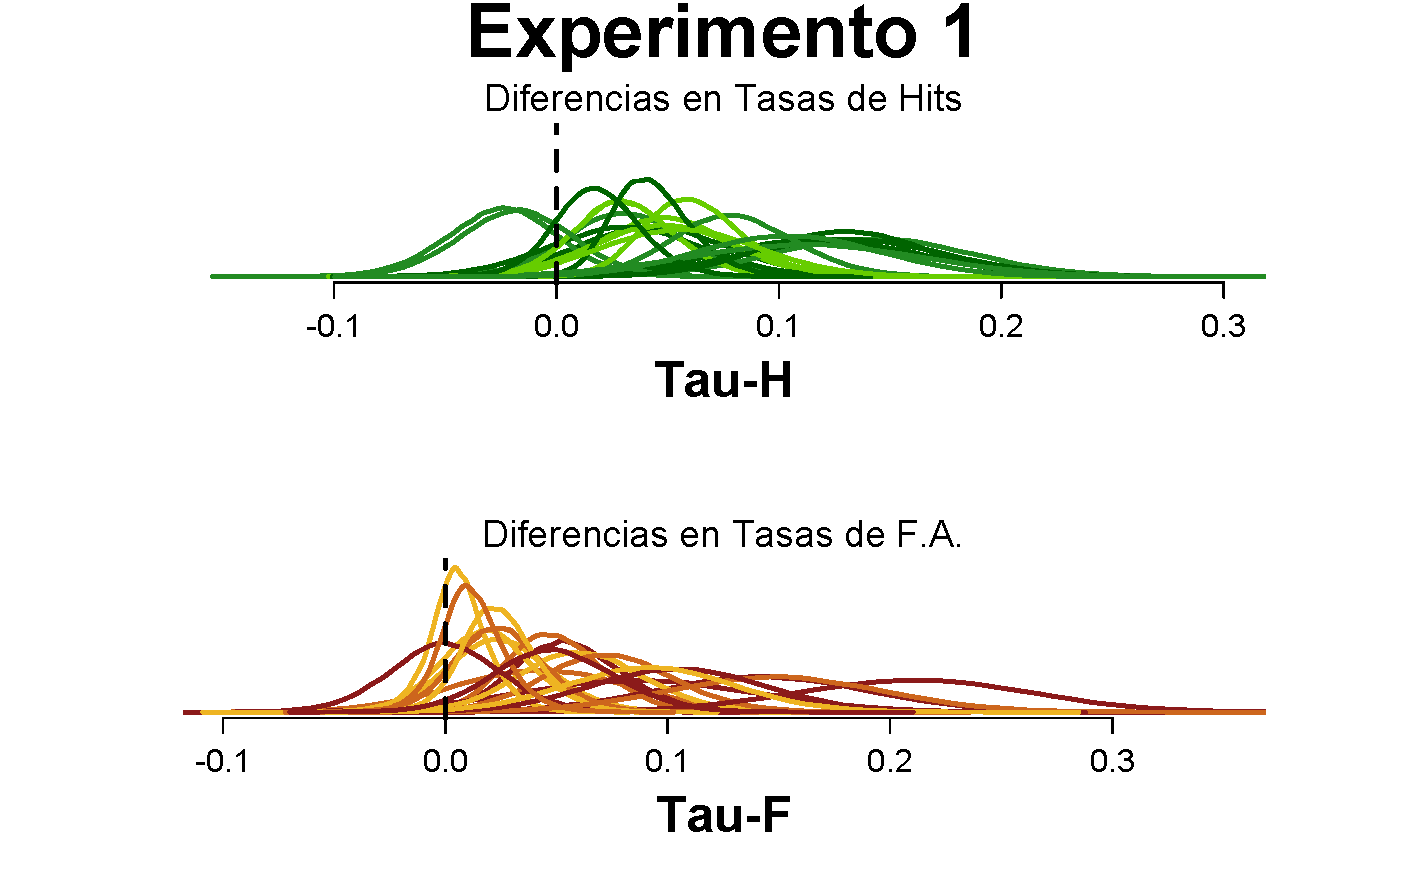
\includegraphics[width=0.8\textwidth]{Figures/Theta_Tau_Post_Ex1}
\end{figure}
\clearpage


---
\begin{figure}[h]
\centering
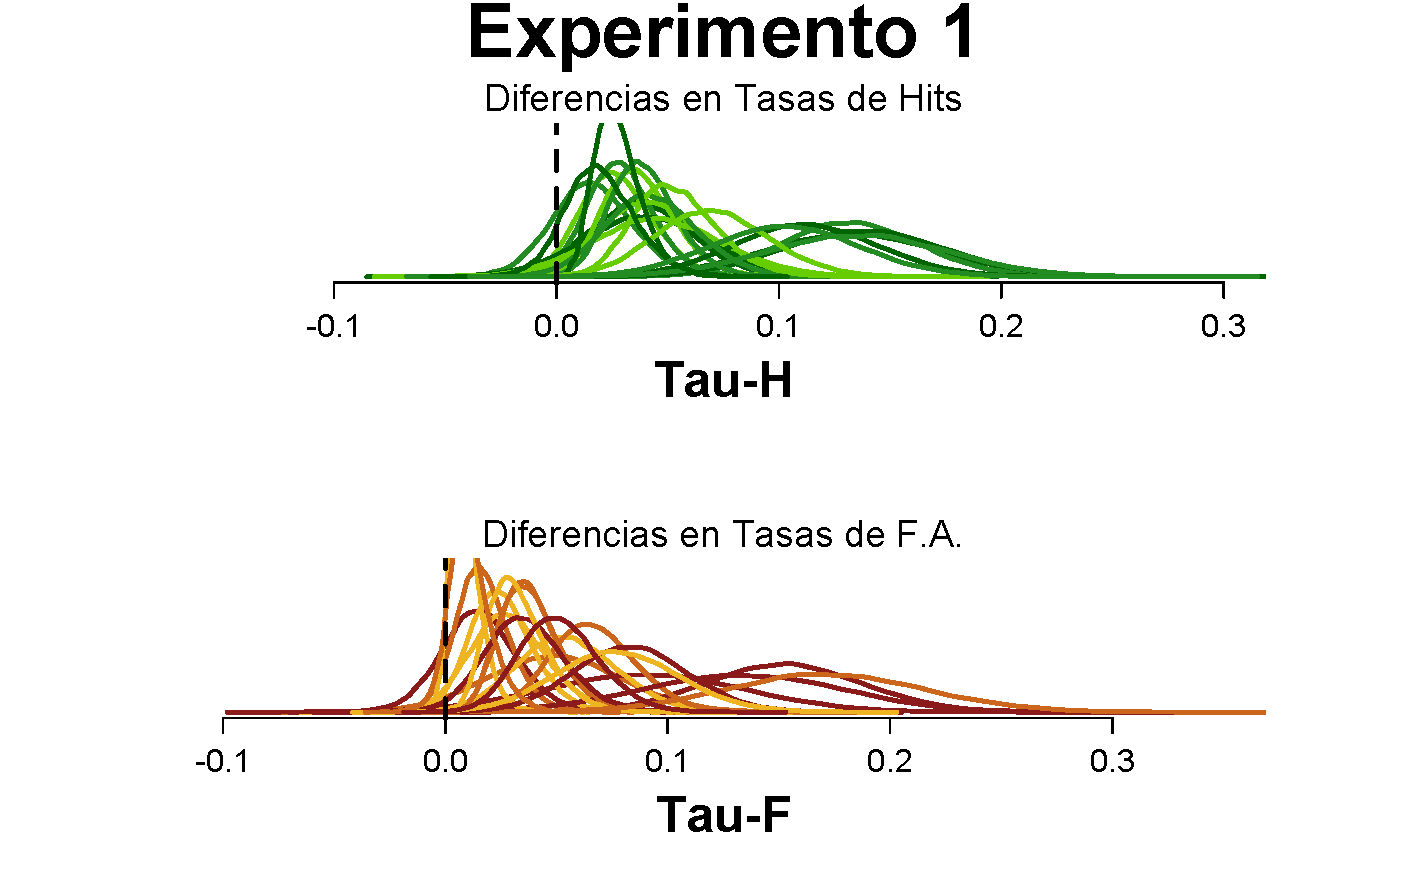
\includegraphics[width=0.8\textwidth]{Figures/Theta_Tau_Post_Cij_Ex1}
\end{figure}
\clearpage

---
\begin{center}
{\LARGE \textbf{Modelo gráfico 2:} }\\
{\small \textsc{(El parámetro Tau estima la diferencia entre las ThetaH y Theta FA))}}\\
\smallskip
\end{center}

\begin{figure}[h]
\centering
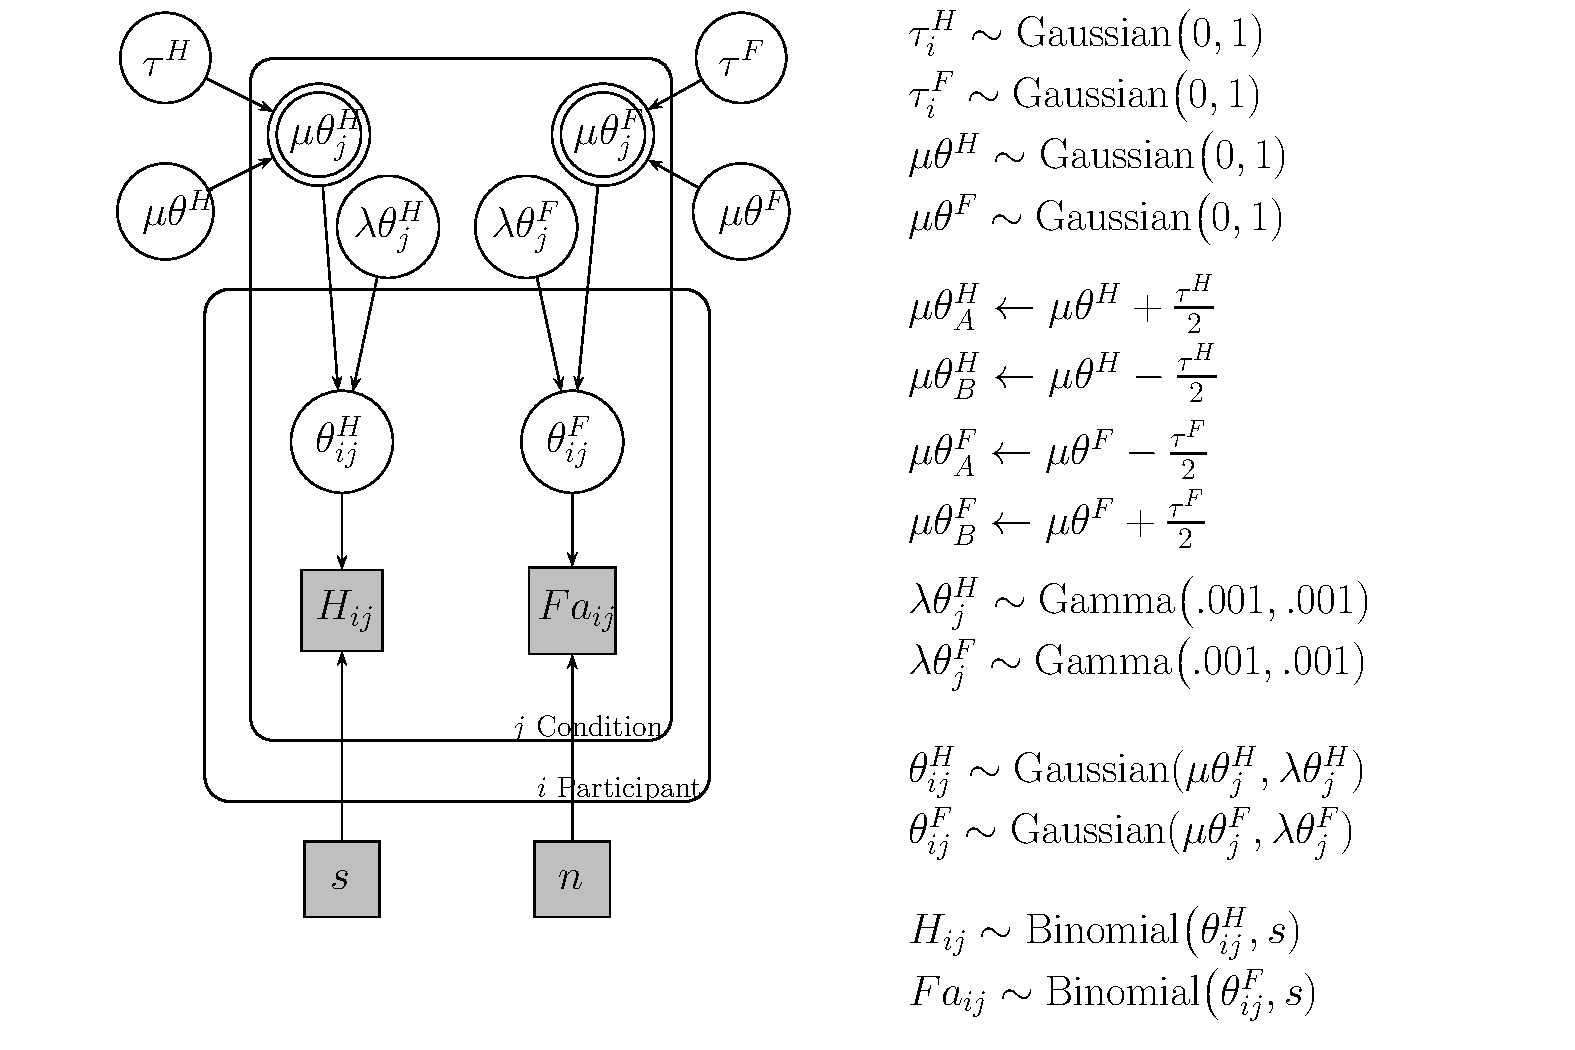
\includegraphics[width=.8\textwidth]{Figures/Theta_BinomialHierarchical}
\end{figure}
\clearpage




---
\begin{figure}[h]
\centering
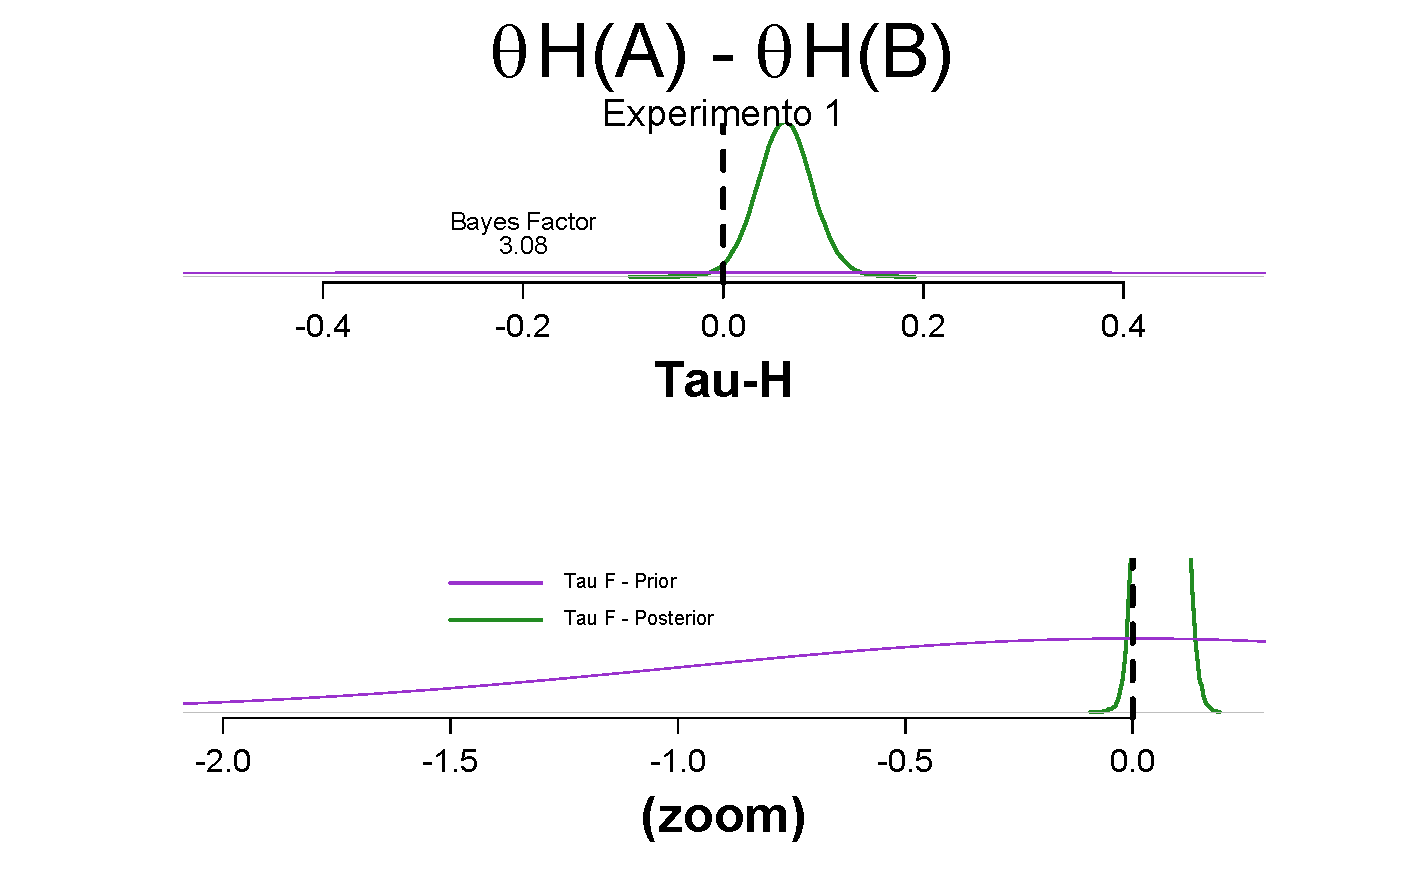
\includegraphics[width=0.8\textwidth]{Figures/Theta_Ro_Exp1_TauH}
\end{figure}
\clearpage


---
\begin{figure}[h]
\centering
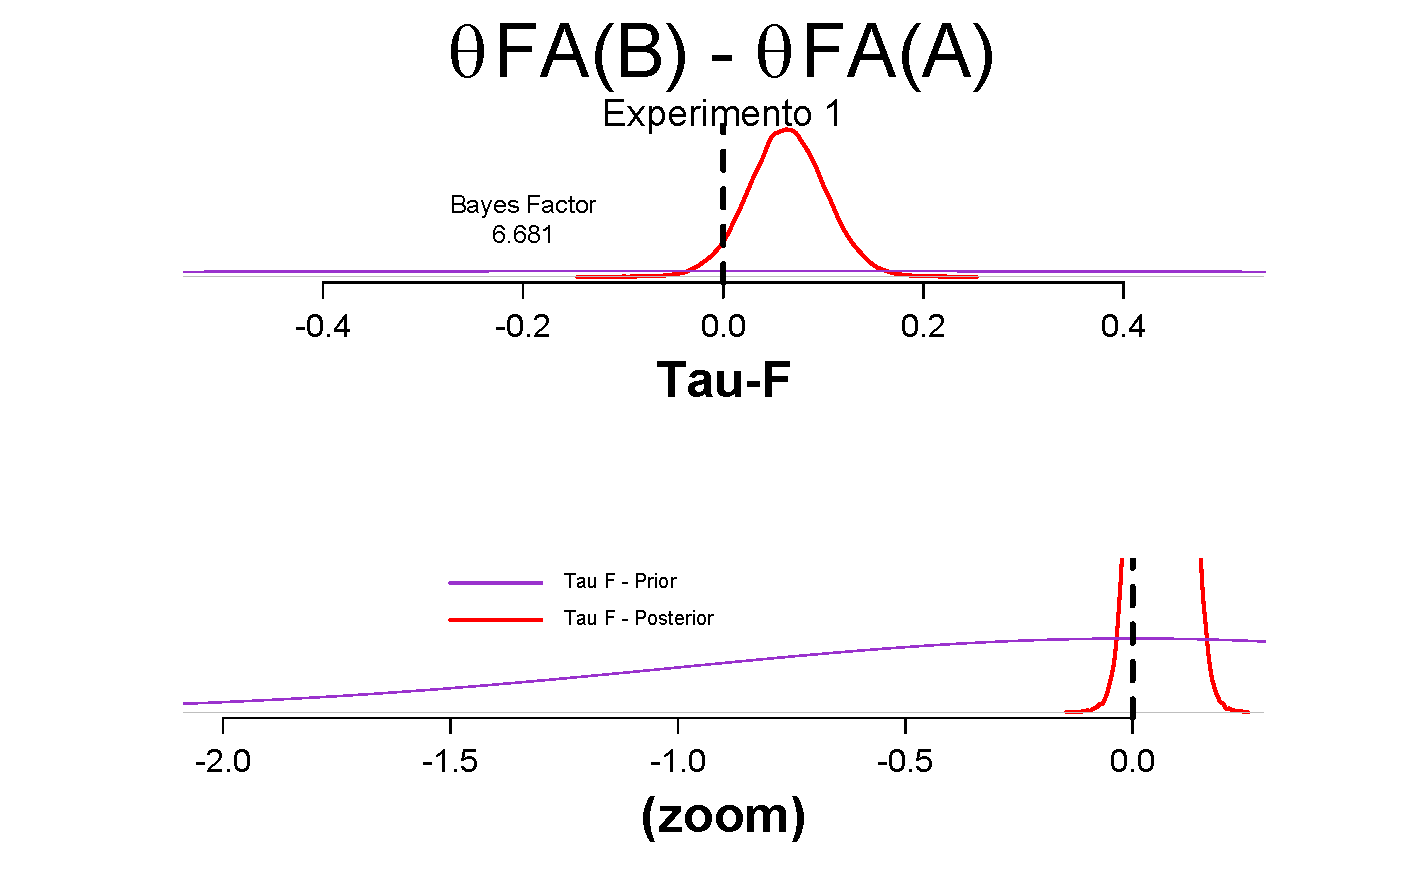
\includegraphics[width=0.8\textwidth]{Figures/Theta_Ro_Exp1_TauFA}
\end{figure}
\clearpage








---
\begin{center}
{\LARGE \textbf{EXPERIMENTO 2} }\\
{\small \textsc{(Figura de Ebbinghaus vs Círculo))}}\\
\smallskip
\end{center}

\begin{figure}[h]
\centering
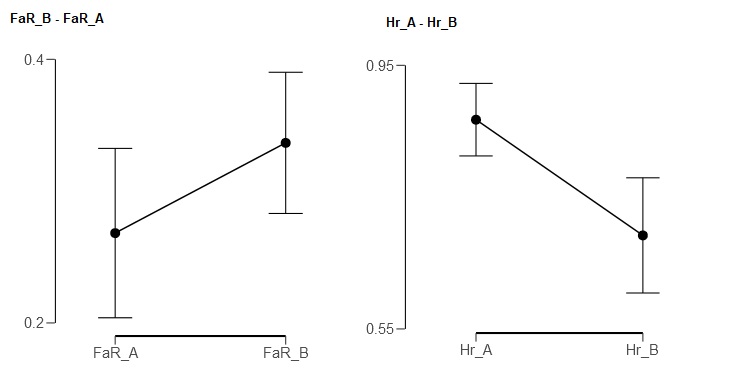
\includegraphics[width=.9\textwidth]{Figures/JASP_Ex2_Dispersion_HyFA}
\end{figure}
\clearpage




---
\begin{figure}[h]
\centering
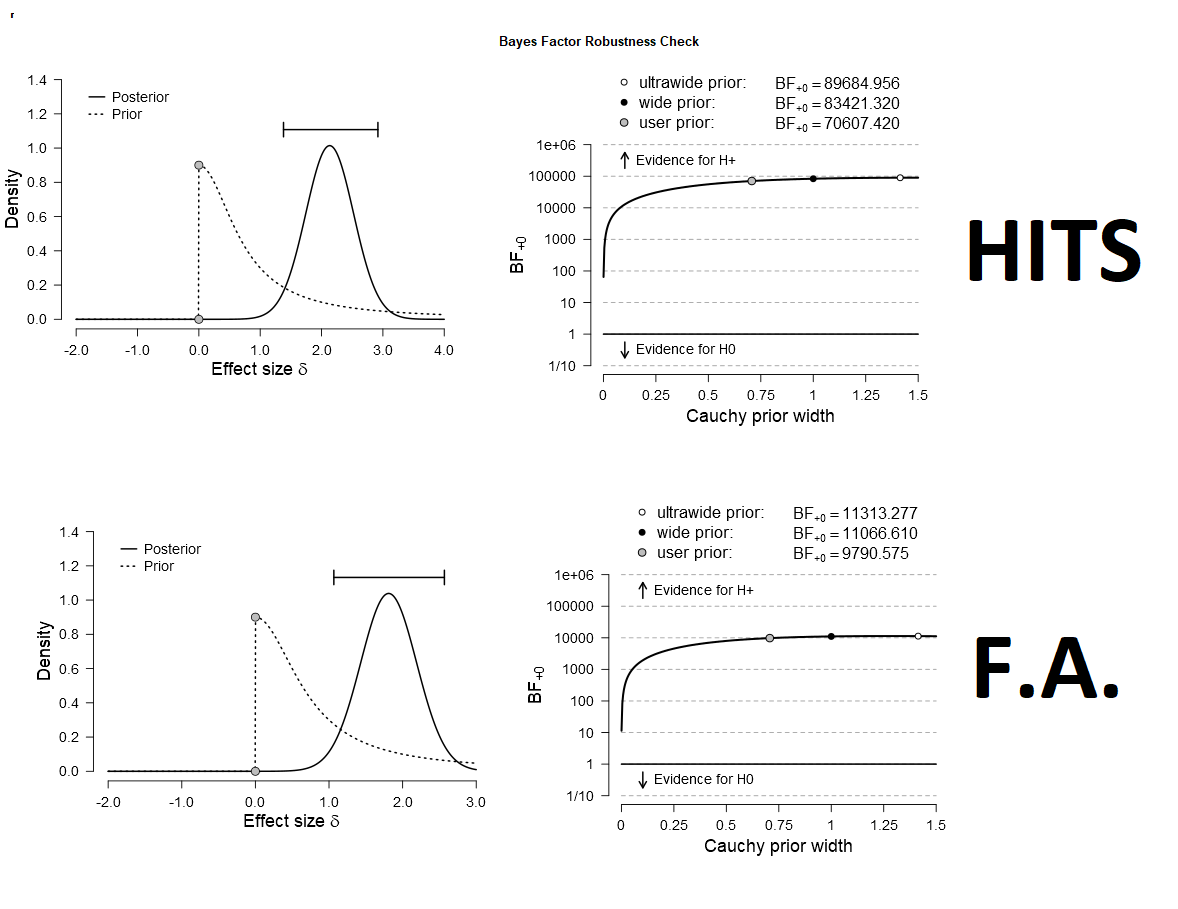
\includegraphics[width=.8\textwidth]{Figures/JASP_Ex2_tTest_HyFA}
\end{figure}
\clearpage





---
\begin{center}
{\LARGE \textbf{Modelo gráfico 1:} }\\
{\small \textsc{(El parámetro Tau estima la diferencia entre las ThetaH y Theta FA))}}\\
\smallskip
\end{center}

\begin{figure}[h]
\centering
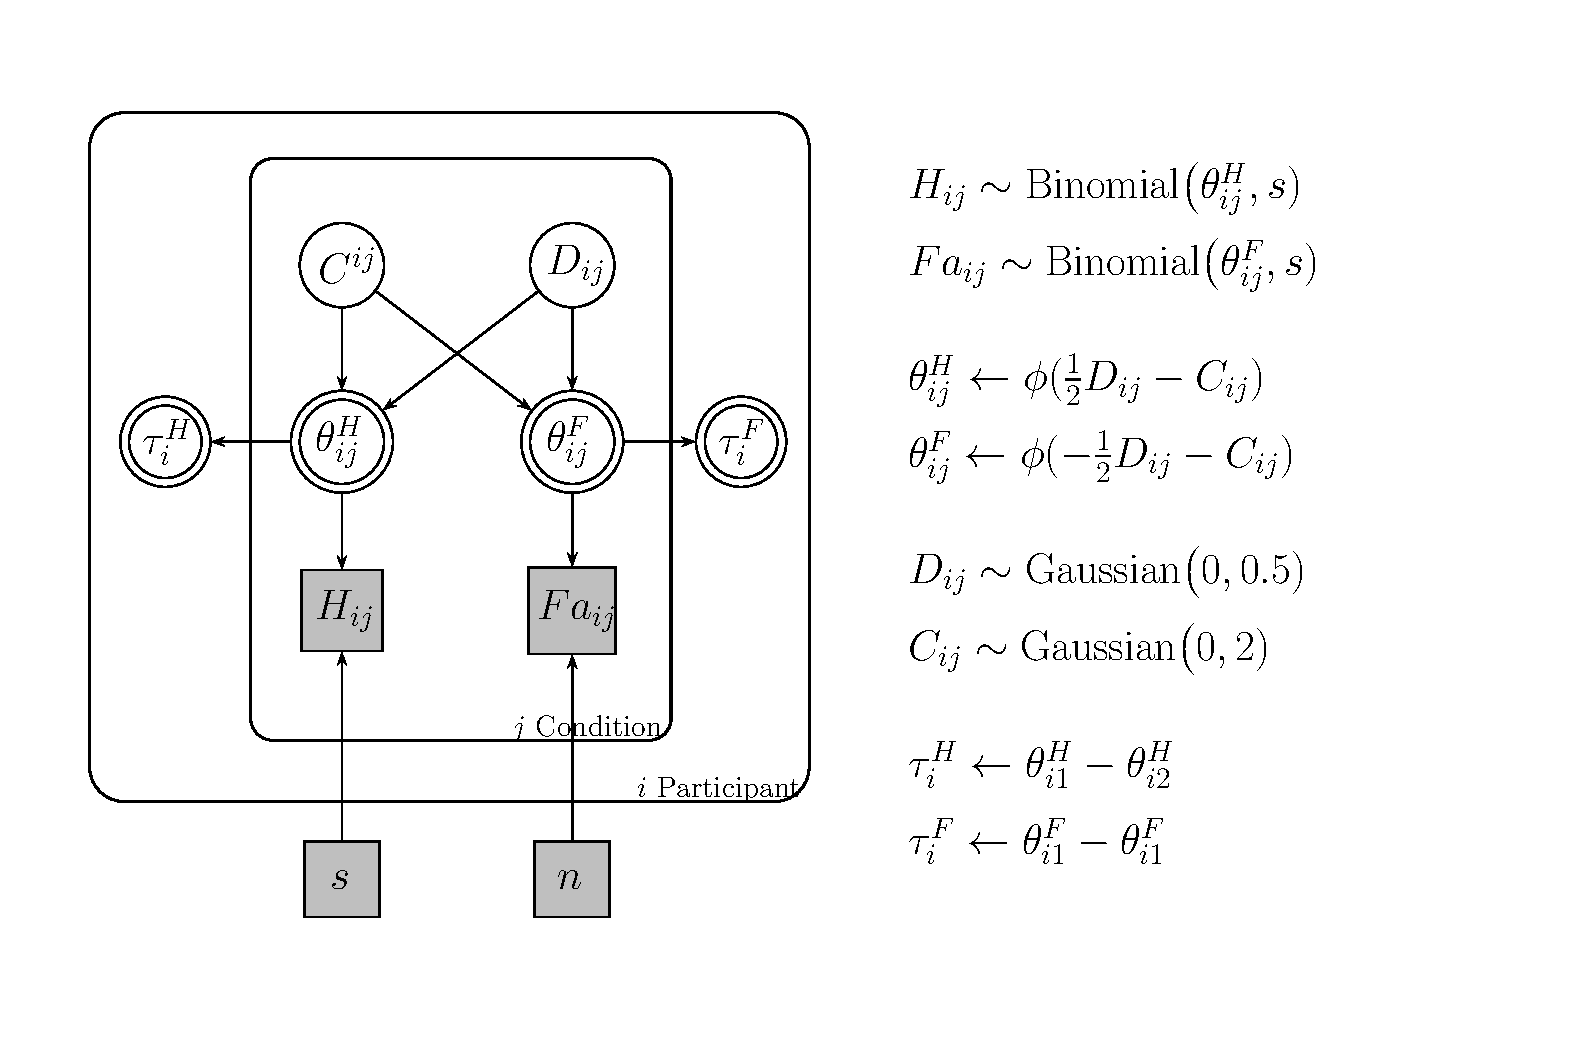
\includegraphics[width=.8\textwidth]{Figures/Theta_Tau}
\end{figure}
\clearpage


---
\begin{figure}[h]
\centering
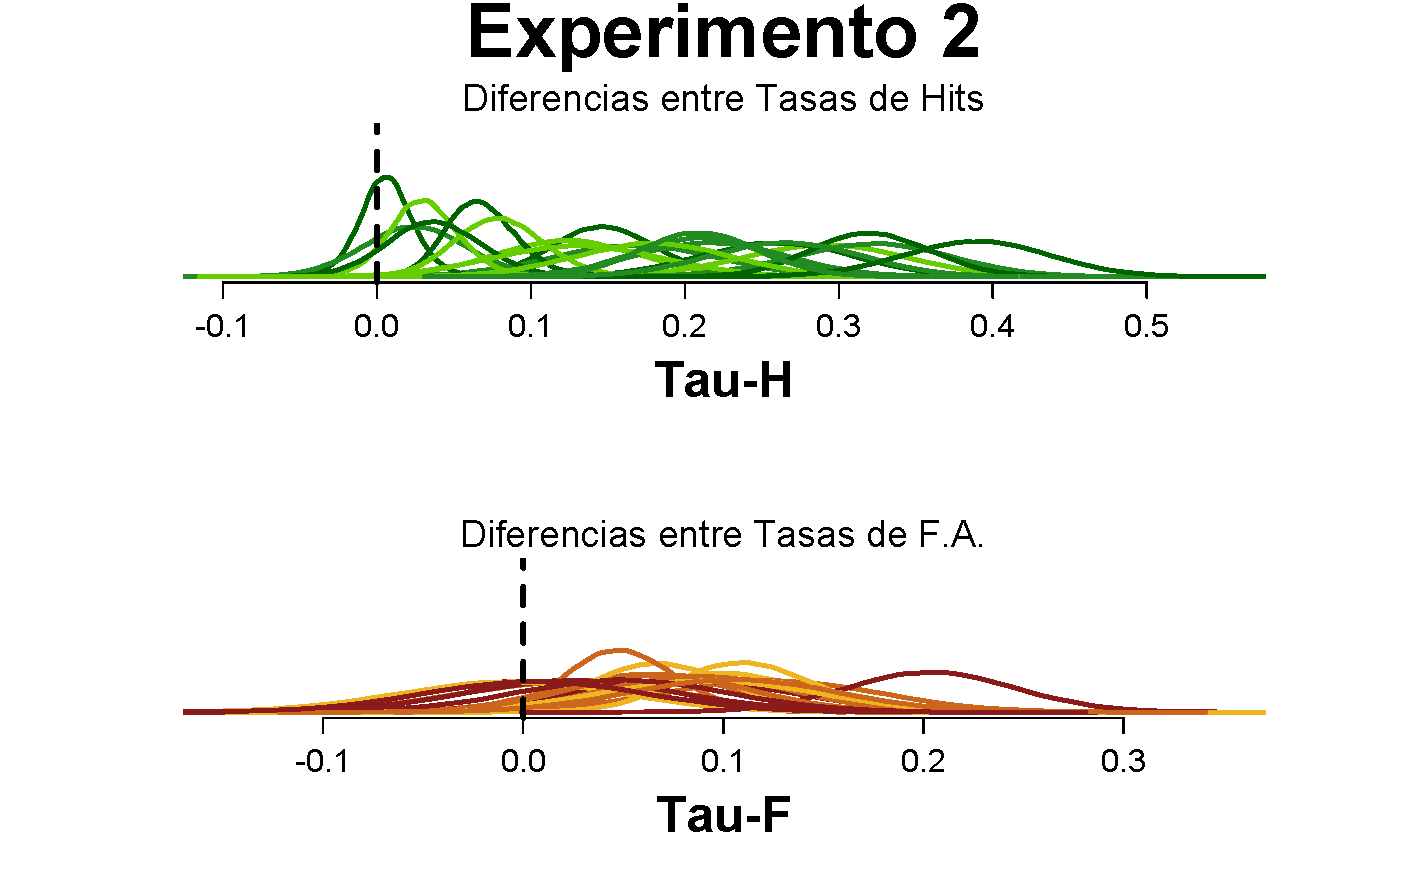
\includegraphics[width=0.8\textwidth]{Figures/Theta_Tau_Post_Cij}
\end{figure}
\clearpage

---
\begin{figure}[h]
\centering
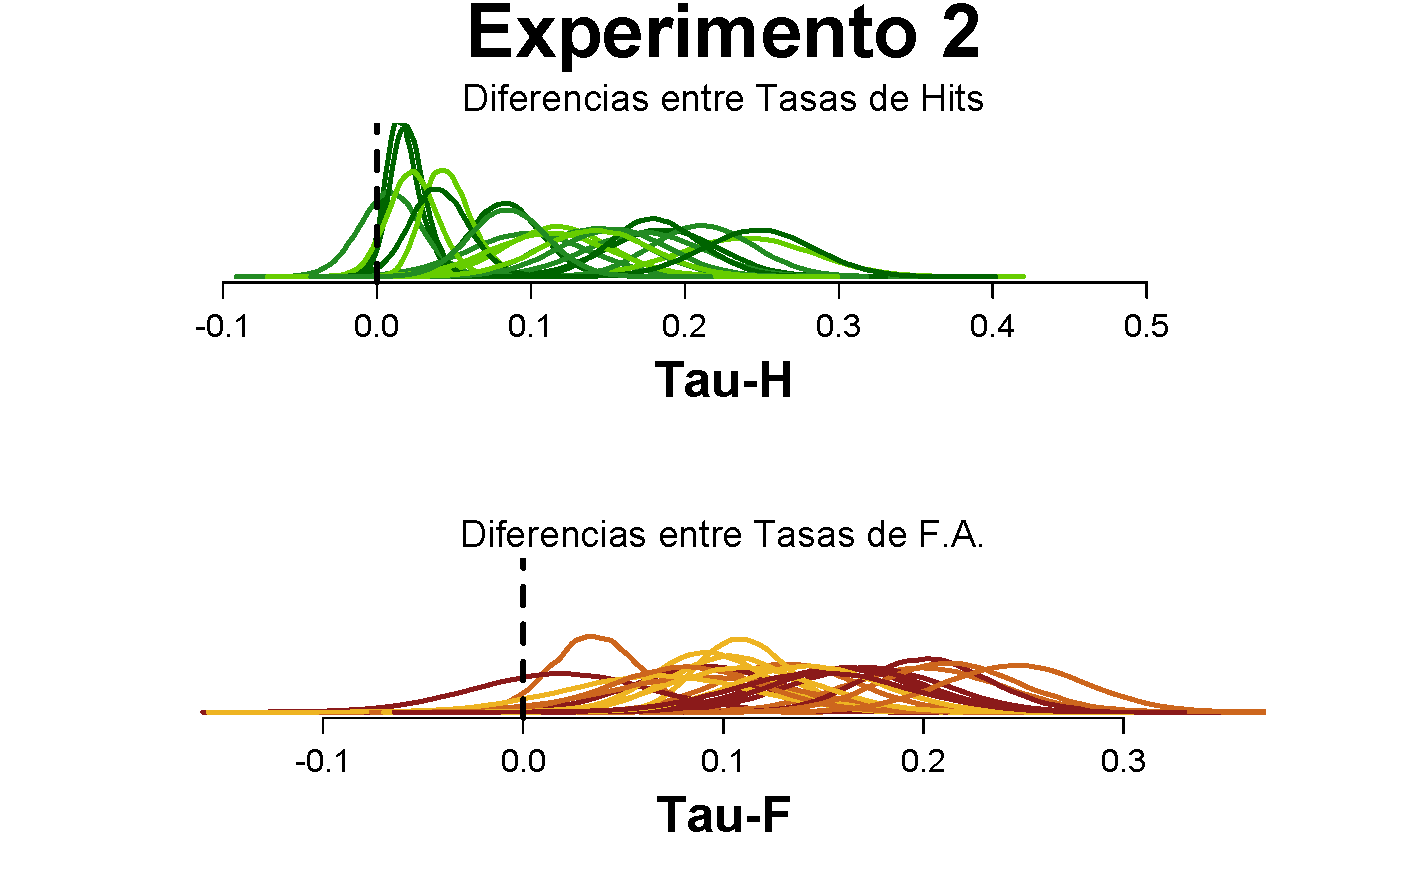
\includegraphics[width=0.8\textwidth]{Figures/Theta_Tau_Post}
\end{figure}
\clearpage




---
\begin{center}
{\LARGE \textbf{Modelo gráfico 2:} }\\
{\small \textsc{(El parámetro Tau estima la diferencia entre las ThetaH y Theta FA))}}\\
\smallskip
\end{center}

\begin{figure}[h]
\centering
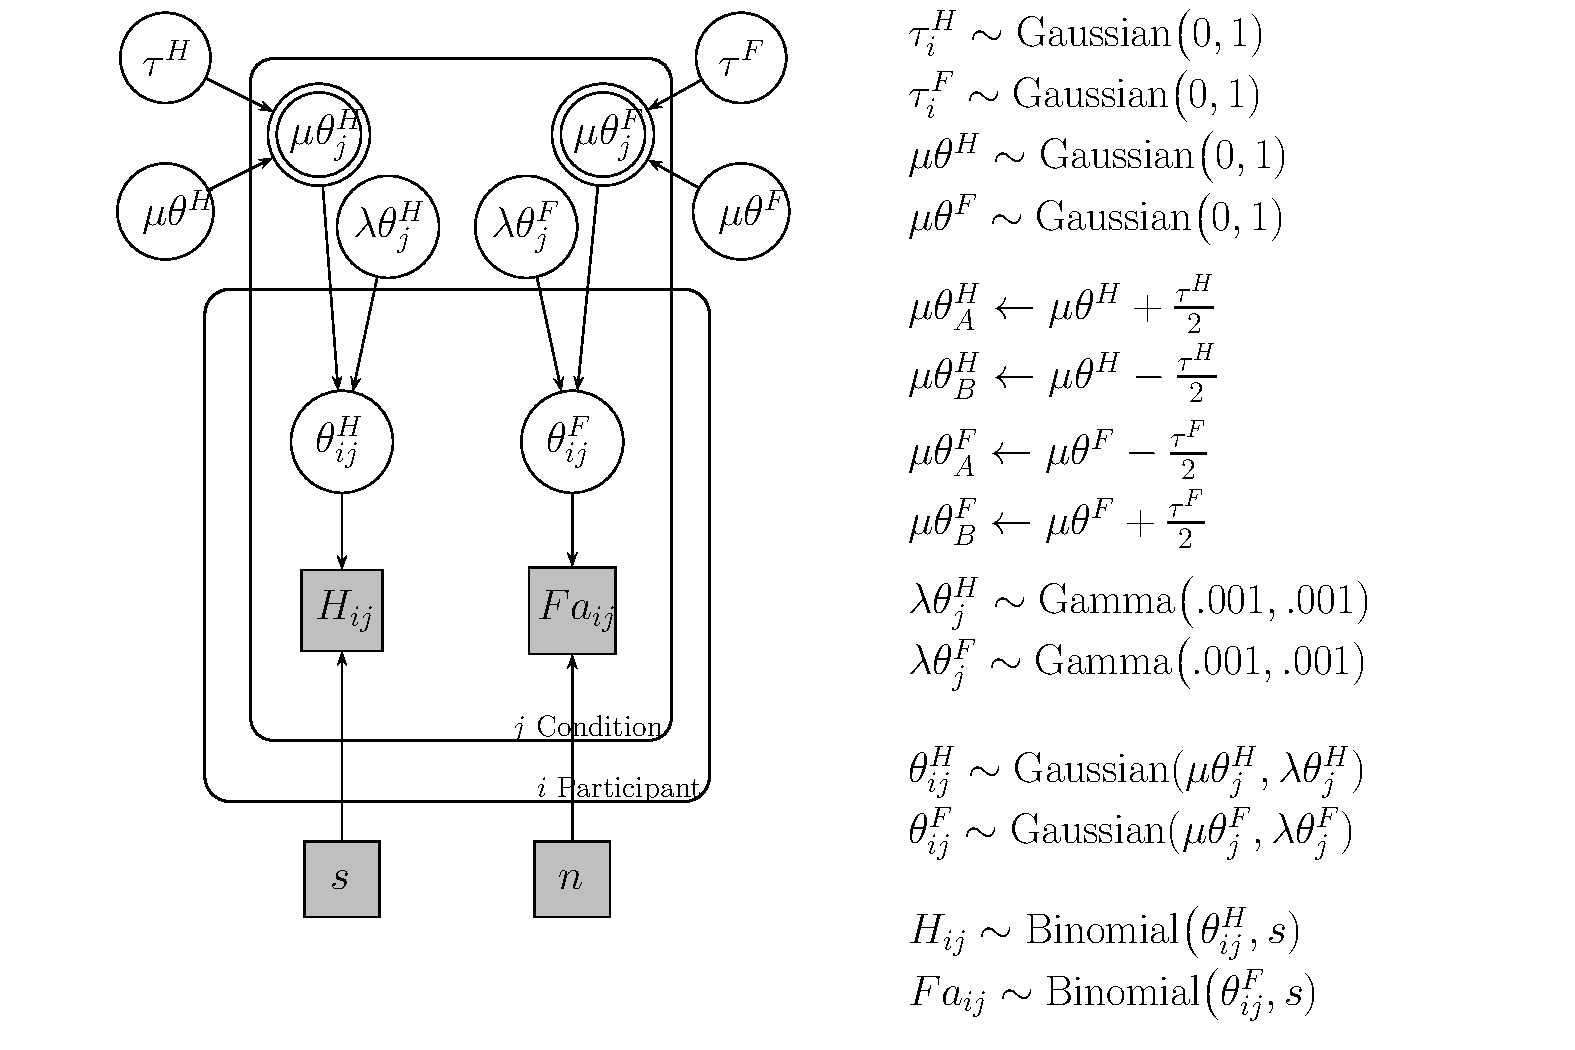
\includegraphics[width=.8\textwidth]{Figures/Theta_BinomialHierarchical}
\end{figure}
\clearpage




---
\begin{figure}[h]
\centering
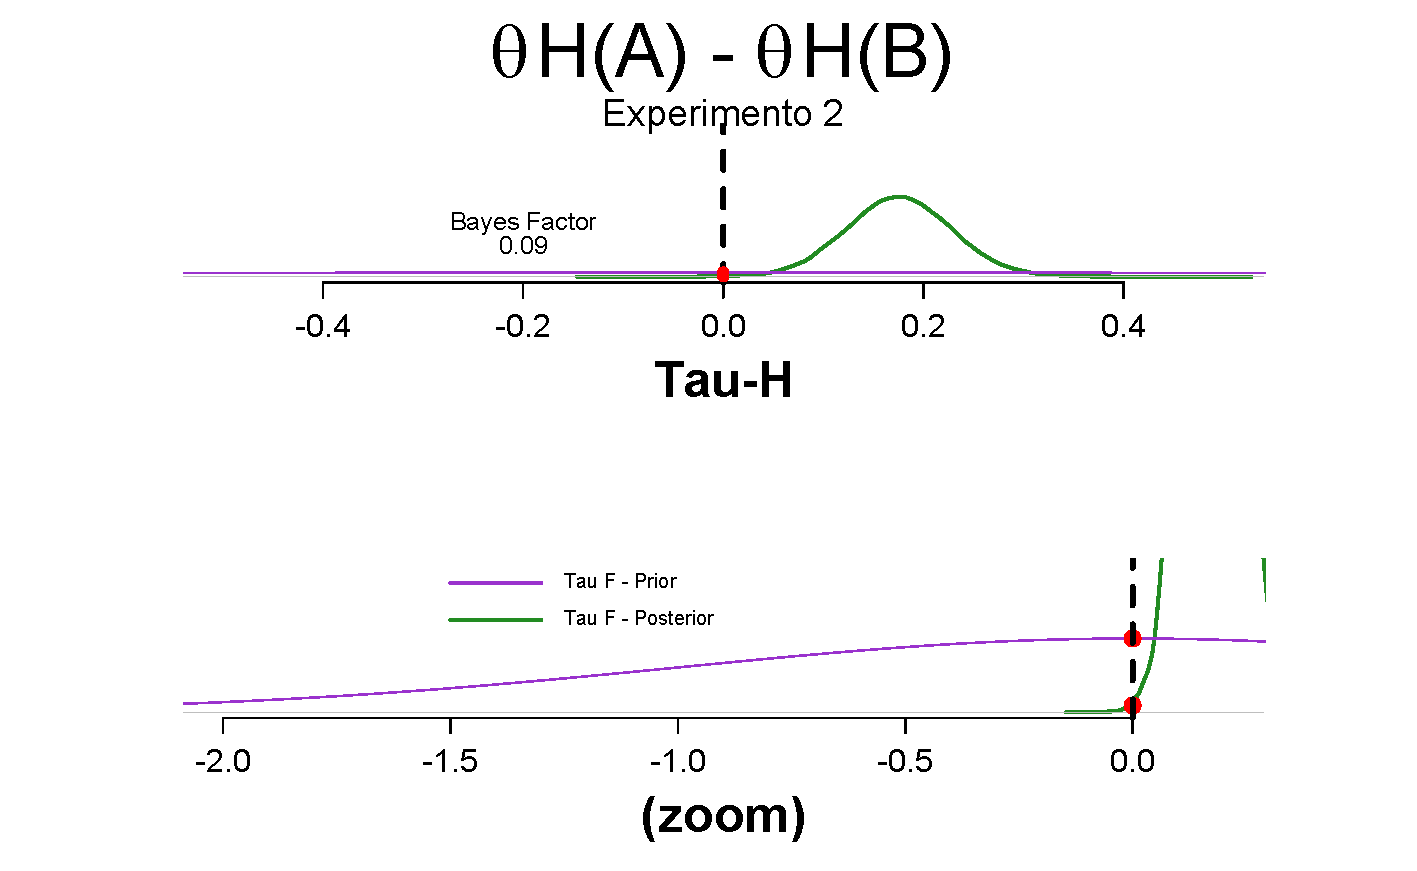
\includegraphics[width=0.8\textwidth]{Figures/Theta_Ro_Exp2_TauH}
\end{figure}
\clearpage


---
\begin{figure}[h]
\centering
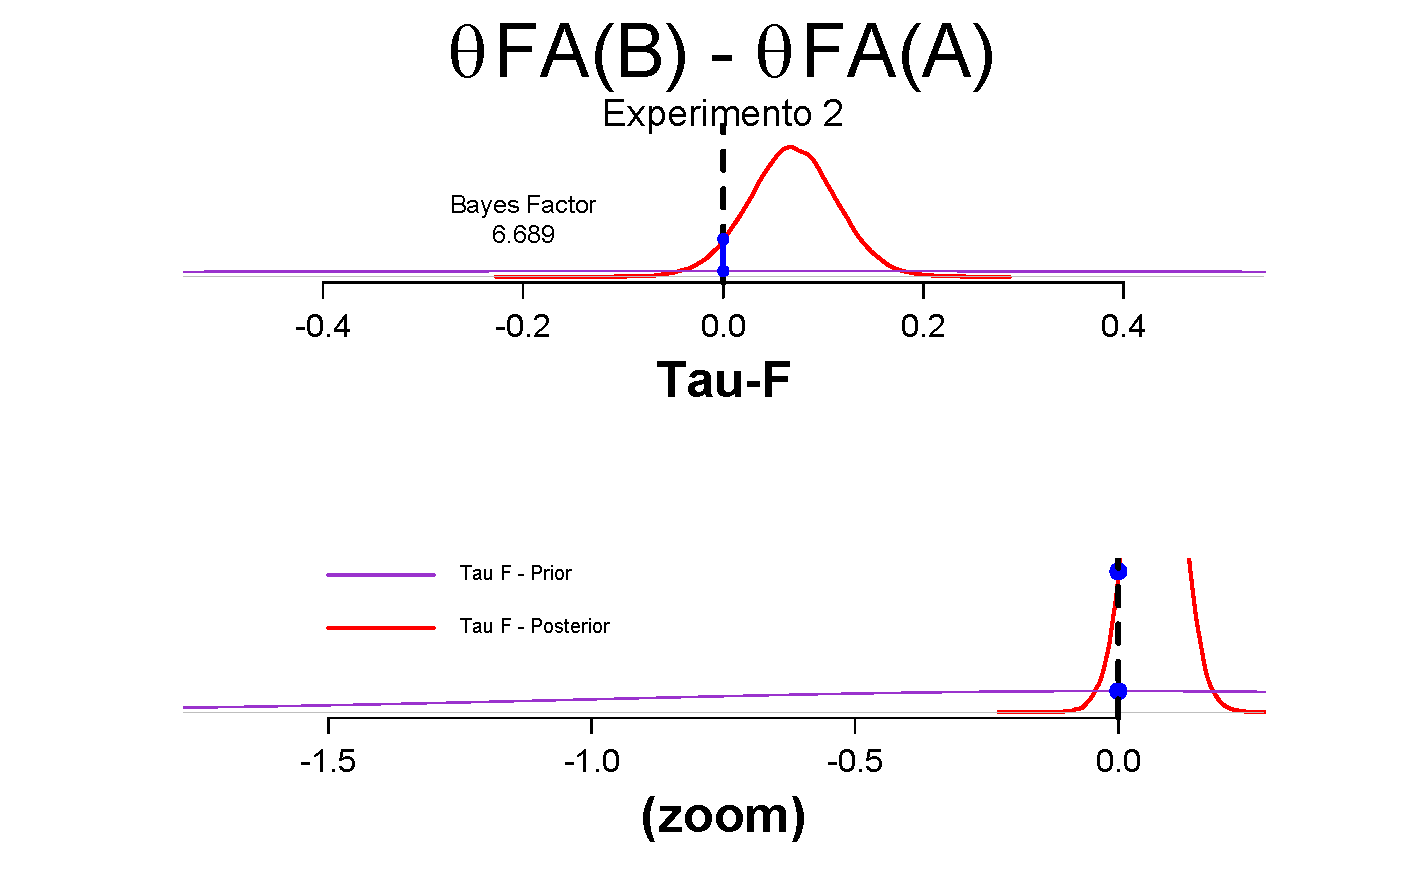
\includegraphics[width=0.8\textwidth]{Figures/Theta_Ro_Exp2_TauFA}
\end{figure}
\clearpage







\end{document}